\subsection{Boundary Continuity of Biholomorphisms}
Suppose \(\Omega_1\) and \(\Omega_2\) are two regions in the complex plane such that there is a biholomorphism \(\varphi\) from \(\Omega_1\) to \(\Omega_2\). Naturally, we are concerned about the existence of a continuous extension of
\(\varphi\) to \(\overline{\Omega_1}\).

In fact, it is almost always true that such an extension exists. We will give three examples of this phenomenon, each with increasing regularity assumptions on the boundaries \(\partial\Omega_1\) and \(\partial\Omega_2\):
\begin{enumerate}
    \item If \(\partial\Omega_1\) and \(\partial\Omega_2\) are two Jordan curves, then \(\varphi\) (whose existence is given by the Riemann Mapping Theorem or \cref{thm:riemannmapping}) extends homeomorphically to
        \(\partial\Omega_1\) (\cref{thm:osgoodtaylorcaratheodory}).
    \item If \(\partial\Omega_1\) and \(\Omega_2\) are \(C^\infty\), then \(\varphi\) extends continuously and injectively to \(\partial\Omega_1\) and is \(C^\infty\) on \(\overline{\Omega_1}\).
    \item If \(\partial\Omega_1\) and \(\partial\Omega_2\) are real-analytic (the boundary is parameterizable by functions such that at every point, there is a power series expansion that converge to the function on a neighborhood), then \(\varphi\) extends analytically past \(\partial\Omega_1\) (\cref{thm:osgoodtaylorcaratheodoryrealanalyticboundaries}).
\end{enumerate}
\begin{example}
    The biholomorphism \(\varphi:\mathbb{D}\to\mathbb{D}\cap\mathbb{H}^+\) defined by \[\varphi:z\mapsto\frac{1+\ii\sqrt{\frac{\ii(1-z)}{1+z}}}{1-\ii\sqrt{\frac{\ii(1-z)}{1+z}}}\] extends continuously but not differentiably to \(\pm1\). The boundary of \(\mathbb{D}\cap\mathbb{H}^+\) is piecewise \(C^\infty\).
\end{example}
\begin{theorem}[name=\textsc{Osgood--Taylor--Carathéodory},store=thm:osgoodtaylorcaratheodory]\label{thm:osgoodtaylorcaratheodory}
    Suppose that \(\Omega_1\) and \(\Omega_2\) are two bounded regions in \(\mathbb{C}\) such that \(\partial\Omega_1\) and \(\Omega_2\) each comprises a single Jordan curve. If \(\varphi:\Omega_1\to\Omega_2\) is a biholomorphism (provided by the Riemann Mapping Theorem in \cref{thm:riemannmapping}), then \(\exists\widetilde{\varphi}:\overline{\Omega_1}\to\overline{\Omega_2}\) homeomorphic such that \(\widetilde{\varphi}{\restriction_{\Omega_1}}\equiv\varphi\) (the restriction of \(\widetilde{\varphi}\) to \(\Omega_1\) agrees with \(\varphi\)).
\end{theorem}
\begin{proof}
    The theorem will be first proven in the case that \(\Omega_1\) is the unit disk \(\mathbb{D}\). The general case will then be reduced to this special case.

    Let \(\mu_1,\mu_2:[0,1]\to\overline{\mathbb{D}}\) be two curves such that \(\mu_1([0,1)),\mu_1([0,1))\subset\mathbb{D}\) and \(\mu_1(1)=1\), \(\mu_2(1)=1\) (as in \cref{fig:osgoodtaylorcaratheodory_unitdiskandVandmu}). We now aim to show that \(\lim_{t\to 1^-}\varphi\qty(\mu_1(t))=\lim_{t\to 1^-}\varphi\qty(\mu_2(t))\) (existence and equality).

    Let \(V=\mathbb{D}\cap D\qty(1,\frac12)\), which has a finite area. Since \(\varphi\) is a biholomorphism, \(\varphi(V)\subset\Omega_2\) also has a finite area (call this \(M\)) and is simply connected since its complement in \(\Omega_2\), \(\varphi\qty(\mathbb{D}\setminus V)\), is connected.

    \begin{figure}
        \centering\vspace{0pt}
        \begin{minipage}{0.45\textwidth}
            \centering
            \vspace{0pt}
            \begin{tikzpicture}
                \draw[thick, name path=A] (-1.875, 0) arc (180:-180:1.875);
                \draw[thick, name path=B] (2.8125, 0) arc (0:360:0.9375);
                \tikzfillbetween[of=A and B,
                split, every segment no 1/.style={pattern=north east lines}]{fill=none};
                \draw[thick, ->] plot[smooth] coordinates {
                    (-0.5, 1.2)(-0.2, 0.8) (0.3,1) (0.6,0.9) (0.8,0.6) (0.9,0.4) (1.3,0.45) (1.875,0)
                };
                \node[anchor=north] at (1.3,0.2) {\(V\)};
                \node[anchor=north] at (-0.4,-0.4) {\(\mu_2\)};
                \node[anchor=north] at (0,0.8) {\(\mu_1\)};
                \node[anchor=north] at (-1.7, -1.2) {\(\partial\mathbb{D}\)};
                \draw[thick, ->] plot[smooth] coordinates {
                    (-0.5, -0.9) (-0.9, -0.8) (-0.3, 0.1) (0.1,-0.5) (0.4,-0.8) (0.8,-0.4) (1.0,-0.5) (1.3,-0.6) (1.875,0)
                };
            \end{tikzpicture}
            \caption{Configuration of \(V\), and possible \(\mu_1,\mu_2\).}
            \label{fig:osgoodtaylorcaratheodory_unitdiskandVandmu}
        \end{minipage}
        \hfill
        \begin{minipage}{0.45\textwidth}
            \centering
            \vspace{0pt}
            \begin{tikzpicture}
                \draw[thick, name path=A] plot[smooth cycle] coordinates {
                    (3.6,0.9) (2.1,2.55) (-1.2,0.75) (-1.5,-0.75) (-1.1,-1.3) (-0.75,-1.5) (0.5,-1.4) (1.65,-1.35)
                };

                \draw[thick, name path=B] plot[smooth] coordinates {
                    (-1.51,-0.751)
                    (-1.1,-0.4) (-0.6,-0.5) (-0.1,0.2) (0.4,0.5)
                    (0.9,0.1) (1.2, -0.2) (1.6499, -1.3501)
                };
                \tikzfillbetween[of=A and B,
                split, every segment no 1/.style={pattern=north east lines}]{fill=none};
                \node[anchor=north] at (0.2, -0.5) {\(\varphi(V)\)};
                \node[anchor=north] at (2.6, -0.8) {\(\partial\Omega_2\)};
            \end{tikzpicture}
            \caption{Possible positioning of \(\varphi(V)\) relative to \(\Omega_2\).}\label{fig:osgoodtaylorcaratheodory_phiofV}
        \end{minipage}
    \end{figure}Let \(K\subset\Omega_2\) be compact. Since \(\varphi^{-1}\) is continuous, it maps \(K\) to a compact set \(\varphi^{-1}(K)\) (a function providing the compactness of the pre-image of every compact set is more generally known as \textit{proper}). This implies that for any sequence \(\cbraces{z_j}_{j\in\mathbb{N}}\subset\mathbb{D}\) with accumulation points only in \(\partial\mathbb{D}\), \(\cbraces{\varphi\qty(z_j)}_{j\in\mathbb{N}}\) will have its accumulation points in \(\partial\Omega_2\) (because otherwise, there would be a corresponding subsequence of \(\cbraces{z_j}_{j\in\mathbb{N}}\) that converges to a point in \(\mathbb{D}\)). Therefore, \(\varphi(V)\) does not have relatively compact closure in \(\Omega_2\) (a representation of a possible configuration in \cref{fig:osgoodtaylorcaratheodory_phiofV}).

    \begin{figure}
        \centering\vspace{0pt}
        \begin{minipage}{0.45\textwidth}
            \centering
            \vspace{0pt}
            \begin{tikzpicture}[>=stealth,
                    arrow style/.style={
                        postaction={decorate},
                        decoration={markings, mark=at position 0.5 with {\arrow[scale=1]{Stealth}}}
                }]
                \draw[thick, name path=A] (-1.875, 0) arc (180:-180:1.875);
                \draw[thick, name path=B] (2.8125, 0) arc (0:360:0.9375);
                \draw[thick, name path=B] (2.8125, 0) arc (0:360:0.9375);
                \draw[thick, name path=C] \tikzcenterarc(1.875,0)(99.1:260.9:0.6);

                %\tikzfillbetween[of=A and B,split, every segment no 1/.style={pattern=north east lines}]{fill=none};
                %\tikzfillbetween[of=A and C,split, every segment no 1/.style={pattern=north west lines}]{fill=none};
                \node[circle, fill=black, inner sep=1pt, label={[xshift=-0.1cm]right:{\small\(1\)}}] at (1.875,0) {};
                \node[anchor=north] at (0.7,0.2) {\small\(V\)};
                \node[anchor=south] at (0,0.7) {\scriptsize\(-\theta_0(r)<\theta<\theta_0(r)\)};
                \node[anchor=south] at (1.8,1.1) {\scriptsize\(-\theta_0(r)\)};
                \node[anchor=north] at (1.8,-1.1) {\scriptsize\(\theta_0(r)\)};
                \node[anchor=north] at (1.5,0.3) {\scriptsize\(\gamma_r\)};
                \node[anchor=north] at (-1.6, -1.2) {\small\(\partial\mathbb{D}\)};
                \draw[-{Stealth}] (1.8,-1.1) -- (1.8,-0.65);
                \draw[-{Stealth}] (1.8,1.1) -- (1.8,0.65);
                \draw[-{Stealth}] (0.3,0.75) -- (1.22,0.1);

            \end{tikzpicture}
            \caption{Possible configuration of \(\gamma_r\).}
            \label{fig:osgoodtaylorcaratheodory_gammarconfiguration}
        \end{minipage}
        \hfill
        \begin{minipage}{0.45\textwidth}
            \centering
            \vspace{0pt}
            \begin{tikzpicture}
                \draw[thick, name path=A] plot[smooth cycle] coordinates {
                    (3.6,0.9) (2.1,2.55) (-1.2,0.75) (-1.5,-0.75) (-1.1,-1.3) (-0.75,-1.5) (0.5,-1.4) (1.65,-1.35)
                };

                \draw[thick, name path=B] plot[smooth] coordinates {
                    (-1.51,-0.751)
                    (-1.1,-0.4) (-0.6,-0.5) (-0.1,0.2) (0.4,0.5)
                    (0.9,0.1) (1.2, -0.2) (1.6499, -1.3501)
                };
                \draw[thick, name path=C] plot[smooth] coordinates {
                    (-1.11,-1.31) (-1,-0.8) (-0.5,-0.9) (-0.2,-0.5) (0.2,-0.7) (0.7, -1.1) (0.5,-1.41)
                };
                %\tikzfillbetween[of=A and B,split, every segment no 1/.style={pattern=north east lines}]{fill=none};
                %\tikzfillbetween[of=A and C,split, every segment no 1/.style={pattern=north west lines}]{fill=none};
                \node[anchor=north] at (0.5, 0.1) {\small\(\varphi(V)\)};
                \node[anchor=north] at (0, -0.7) {\footnotesize\(\varphi\qty(\gamma_r)\)};
                \node[anchor=north] at (2.6, -0.8) {\small\(\partial\Omega_2\)};
            \end{tikzpicture}
            \caption{Concept configuration of \(\varphi\qty(\gamma_r)\)}\label{fig:osgoodtaylorcaratheodory_subwedgeimage}
        \end{minipage}
    \end{figure}For \(0<r<\frac12\), we now introduce polar coordinates \((r,\theta)\) centered at \(1\) with angles offset by \(\uppi\). Let \(\theta_0(r)\) be the supremum of \(\theta\) for fixed \(r\) such that \(1-r\ee^{\ii\theta}\in V\). Define \(\gamma_r:\qty(-\theta_0(r),\theta_0(r))\to V\) to be the curve with \(\theta\mapsto 1-r\ee^{\ii\theta}\) (as in \cref{fig:osgoodtaylorcaratheodory_gammarconfiguration}).
    \begin{lemma}\label{lem:osgoodtaylorcaratheodory_lengthintegralfiniteness}
        Let \(l_r\) be the length of \(\varphi\circ\gamma_r\). Then \[\int_0^{\frac12}\frac{l_r^2}{\uppi r}\dd{r}\] is finite.
    \end{lemma}
    \begin{proof}
        Notice that \[l_r=\mathmakebox[\widthof{\(\int_{\varphi\circ\gamma_r\qty(\qty[-\theta_0(r),\theta_0(r)])}\)}][l]{\mathmakebox[\widthof{\(\int\)}][l]{\int_{\varphi\circ\gamma_r\qty(\qty[-\theta_0(r),\theta_0(r)])}}\qquad\abs{\ddz}}=\int_{-\theta_0(r)}^{\theta_0(r)}\abs{\dv{\theta}\varphi\qty(1-r\ee^{\ii\theta})}\dd{\theta}=\int_{-\theta_0(r)}^{\theta_0(r)}r\abs{\varphi'\qty(1-r\ee^{\ii\theta})}\dd{\theta}.\] Hence,
        \begin{align*}
            \int_0^{\frac12}\frac{l_r^2}{\uppi r}\dd{r} & =&&\hspace{-2.5em}\int_0^{\frac12}\frac{1}{\uppi r}\qty[\int_{-\theta_0(r)}^{\theta_0(r)}\abs{\varphi'\qty(1-r\ee^{\ii\theta})}r\dd{\theta}]^2\dd{r}\\
            &=&&\hspace{-2.5em}\int_0^{\frac12}\frac{1}{\uppi r}\qty[\int_{-\theta_0(r)}^{\theta_0(r)}\abs{\varphi'\qty(1-r\ee^{\ii\theta})}\sqrt{r}\sqrt{r}\dd{\theta}]^2\dd{r}\\
            &\mathrel{\phantom{\mathord{\leq}}\mathord{\underset{\substack{\mathllap{\text{Cauchy}}\\\mathllap{\text{Schwarz}}}}{\mathllap{\leq}}}}&&\hspace{-2.5em}\int_0^{\frac12}\frac{1}{\uppi r}\qty[\int_{-\theta_0(r)}^{\theta_0(r)}\abs{\varphi'\qty(1-r\ee^{\ii\theta})}^2 r\dd{\theta}]\qty[\int_{-\theta_0(r)}^{\theta_0(r)}r\dd{\theta}]\dd{r}\\
            &\leq&&\hspace{-2.5em}\int_0^{\frac12}\int_{-\theta_0(r)}^{\theta_0(r)}\abs{\varphi'\qty(1-r\ee^{\ii\theta})}^2 r\dd{\theta}\dd{r}\\
            &=&&\hspace{-2.5em}\iint_V\abs{\varphi'(z)}^2\dd{A}=M,
        \end{align*}
        where the last step uses the Jacobian matrix (see \cref{thm:lusinarea}).
    \end{proof}
    Assume that \(\exists c>0,\varepsilon>0\) such that \(l_r\geq c\) for all \(0<r<\varepsilon\). Then, this implies that \[\int_0^{\frac12}\frac{l_r^2}{\uppi r}\dd{r}\geq\int_0^{\varepsilon}\frac{l_r^2}{\uppi r}\dd{r}\geq\int_0^{\varepsilon}\frac{c^2}{\uppi r}\dd{r}=\frac{c^2}{\uppi}\int_0^\varepsilon\frac{\dd{r}}r,\] which is a divergent integral. This contradicts \cref{lem:osgoodtaylorcaratheodory_lengthintegralfiniteness}. Therefore, we must have \(\varliminf_{r\to 0^+}l_r=0\). Thus, there exists a sequence \(\cbraces{r_j}_{j\in\mathbb{N}}\subset\qty(0,\frac12)\) such that \(r_j\to 0\) and \(l_{r_j}\to 0\) as \(j\to\infty\).
    \begin{proposition}\label{prop:osgoodtaylorcaratheodory_limitsexistence}
        For each such \(r_j\) as above, the limits \[\lim_{\theta\to\theta_0(r_j)^-}\varphi\qty(1-r_j\ee^{\ii\theta})\qand\lim_{\theta\to-\theta_0(r_j)^+}\varphi\qty(1-r_j\ee^{\ii\theta})\] exist.
    \end{proposition}
    \begin{proof}
        Since \(l_{r_j}\) is finite, \(\forall\varepsilon>0\), \(\exists\delta>0\) such that for \(\theta>\theta_0\qty(r_j)-\delta\), \[\int_\theta^{\theta_0\qty(r_j)}r\abs{\varphi'\qty(1-r\ee^{\ii\vartheta})}\dd{\vartheta}.\] Then for any \(\theta',\theta''\in\qty(\theta_0(r)-\delta,\theta_0(r))\),
        \begin{align*}
            \abs{\varphi\qty(1-r\ee^{\ii\theta'})-\varphi\qty(1-r\ee^{\ii\theta''})}&\leq\operatorname{length}\qty(\varphi\qty(\gamma_r\qty([\theta', \theta'']))) \\
            &= \int_{\theta'}^{\theta''}r\abs{\varphi'(1-r\ee^{\ii\vartheta})}\dd{\vartheta}< \varepsilon,
        \end{align*}
        implying that \(\cbraces{\varphi\qty(1-r\ee^{\ii\theta})}_{\theta\to\theta_0(r_j)^-}\) is Cauchy and hence convergent. The proof for the other limit follows symmetrically.
    \end{proof}
    \begin{lemma}\label{lem:osgoodtaylorcaratheodory_jordancurvearcdiameter}
        Let \(\tau=\partial\Omega_2\). Then there is a function \(\eta(\delta)\) defined for sufficiently small \(\delta\), such that \(\eta(\delta)\to 0\) as \(\delta\to 0^+\), such that for all \(a,b\in\tau\) satisfying \(\abs{a-b}\le\delta\), then there is exactly one curve in \(\tau\) with endpoints \(a\) and \(b\) with diameter \(\leq\eta(\delta)\).
    \end{lemma}
    \begin{proof}
        Since \(\tau\) is a Jordan curve, it admits a homeomorphic parametrization \(\psi:S^1\to\tau\), and \(\psi\) is a bicontinuous bijection (onto its image) between compact Hausdorff spaces, so \(\psi^{-1}\) is continuous.

        Since \(\psi^{-1}\) is uniformly continuous on the compact set \(\tau\), for every \(\varepsilon>0\) there exists \(\delta'>0\) such that if \(\abs{p-q}<\delta'\) with \(p,q\in\tau\), then \(\abs{\psi^{-1}(p)-\psi^{-1}(q)}<\varepsilon\).

        In particular, choose \(\delta_0>0\) small enough so that whenever \(\abs{\psi(\zeta)-\psi(\zeta')}\leq\delta_0\), then \(\abs{\zeta-\zeta'}<2\).

        Now define
        \[\eta(\delta)=\sup\cbraces{\diam\rho}{\abs{\psi(\zeta)-\psi(\zeta')}\leq\delta}\]
        for \(0<\delta\leq\delta_0\), where \(\rho=\psi(\sigma)\) and \(\sigma\subseteq S^1\) is the shorter arc connecting \(\zeta,\zeta'\in S^1\).

        First, \(\eta(\delta)\to0\) as \(\delta\to0^+\); if not, there exists \(\varepsilon>0\) and a sequence \(\delta_n\to0^+\) with \(\eta\qty(\delta_n)\geq\varepsilon\). Then for each \(n\in\mathbb{N}\), there are \(\zeta_n,\zeta_n'\in S^1\) with \(\abs{\psi(\zeta_n)-\psi(\zeta_n')}\leq\delta_n\) such that the shorter arc on \(S^1\) between \(\zeta_n\) and \(\zeta_n'\) has image \(\rho_n\) with \(\diam\rho_n\geq\varepsilon\). By compactness of \(S^1\), we may assume (by passing to a subsequence if necessary) that \(\zeta_n\to\zeta\) and \(\zeta_n'\to\zeta'\). Then \(\psi(\zeta)=\lim_{n\to\infty}\psi(\zeta_n)=\lim_{n\to\infty}\psi(\zeta_n')=\psi(\zeta')\), so \(\zeta=\zeta'\). But then the images of the shorter arcs between each \(\zeta_n\) and \(\zeta_n'\) must have diameters tending to zero (by continuity of \(\psi\)), contradicting that \(\diam\rho_n\geq\varepsilon\) for each \(n\).

        To finish, choose \(0 < \delta_1 < \delta_0\) small enough that \(\eta(\delta_1) < \frac{1}{2} \diam \tau\) (possible since \(\eta(\delta) \to 0\) as \(\delta \to 0\) and \(\diam \tau > 0\)).

        Then the assertion holds for all \(\delta\leq\delta_1\) with this \(\eta\): for \(a,b\in\tau\) with \(\abs{a-b}\leq\delta\leq\delta_1\), let \(\zeta,\zeta'\in S^1\) with \(\psi(\zeta)=a\), \(\psi\qty(\zeta')=b\). The shorter arc on \(S^1\) between \(\zeta,\zeta'\) has image \(\rho\) with \(\diam\rho\leq\eta(\delta)\). The image of the other arc on \(\tau\), \(\widetilde{\rho}\) between \(a,b\) satisfies \[\diam\widetilde{\rho}+\diam\rho\geq\diam\tau,\] which is sufficient to imply that \[\diam\widetilde{\rho}\geq\diam\tau-\diam\rho>\diam\tau-\frac12\diam\tau=\frac12\diam\tau>\eta(\delta).\] Thus, exactly one arc's image (specifically, the image of the shorter arc on \(S^1\)) has diameter \(\leq\eta(\delta)\).
    \end{proof}
    By the uniqueness as described by \cref{lem:osgoodtaylorcaratheodory_jordancurvearcdiameter}, for any two points \(a,b\) sufficiently close together, we now identify the unique curve in \(\tau\) (joining \(a\) and \(b\)) with diameter less than \(\eta(\abs{a-b})\) as the \textit{smaller arc} of \(\tau\) joining \(a\) and \(b\), denoted by \(\tau_{a,b}\).
    \begin{lemma}\label{lem:osgoodtaylorcaratheodory_twoalternatives}
        \begin{figure}
            \centering
            \vspace{0pt}
            \begin{tikzpicture}
                \draw[thick, name path=A] plot[smooth cycle] coordinates {
                    (3.6,0.9) (2.1,2.55) (-1.2,0.75) (-1.5,-0.75) (-1.1,-1.3) (-0.75,-1.5) (0.5,-1.4) (1.65,-1.35)
                };

                \draw[thin, name path=B] plot[smooth] coordinates {
                    (-1.51,-0.751)
                    (-1.1,-0.4) (-0.6,-0.5) (-0.1,0.2) (0.4,0.5)
                    (0.9,0.1) (1.2, -0.2) (1.6499, -1.3501)
                };
                \draw[thick, name path=C] plot[smooth] coordinates {
                    (-1.11,-1.31) (-1,-0.8) (-0.5,-0.9) (-0.2,-0.5) (0.2,-0.7) (0.7, -1.1) (0.5,-1.41)
                };
                \node[anchor=north] at (0.2, 0.1) {\footnotesize\(\varphi\qty(\gamma_{r_j})\)};
                \node[anchor=north] at (-1.1,-1.3) {\footnotesize\(a_j\)};
                \node[anchor=north] at (0.5,-1.35) {\footnotesize\(b_j\)};
            \end{tikzpicture}\hfill
            \begin{tikzpicture}
                \draw[thick, name path=A] plot[smooth cycle] coordinates {
                    (3.6,0.9) (2.1,2.55) (-1.2,0.75) (-1.5,-0.75) (-1.1,-1.3) (-0.75,-1.5) (0.5,-1.4) (1.65,-1.35)
                };

                \draw[thin, name path=B] plot[smooth] coordinates {
                    (-1.51,-0.751)
                    (-1.1,-0.4) (-0.6,-0.5) (-0.1,0.2) (0.4,0.5)
                    (0.9,0.1) (1.2, -0.2) (1.6499, -1.3501)
                };
                \draw[thick, name path=C] plot[smooth] coordinates {
                    (-0.75,-1.51) (-0.8,-1.1) (-0.5,-0.9) (-0.2,-0.5) (0.2,-0.7) (0.6, -0.9) (0.4,-1.0) (0.4,-1.2) (-0.75,-1.51)
                };
                \node[anchor=north] at (0.3,0.05) {\footnotesize\(\varphi\qty(\gamma_{r_j})\)};
                \node[anchor=north] at (-0.75,-1.51) {\footnotesize\(p_j\)};
            \end{tikzpicture}
            \caption{Two possibilities for the endpoints of \(\varphi\qty(\gamma_{r_j})\)}\label{fig:osgoodtaylorcaratheodory_curveimagetwocases}
        \end{figure}Let \(\cbraces{r_j}_{j\in\mathbb{N}}\) be the sequence such that \(l_{r_j}\to 0\) as \(j\to\infty\) (in the discussion preceding \cref{prop:osgoodtaylorcaratheodory_limitsexistence}). Then, for each \(j\in\mathbb{N}\), either
        \begin{equation}
            \Omega_2\ni a_j=\lim_{\theta\to\theta_0(r_j)^-}\varphi\qty(1-r_j\ee^{\ii\theta})\neq\lim_{\theta\to-\theta_0\qty(r_j)^+}\varphi\qty(1-r_j\ee^{\ii\theta})=b_j\in\partial\Omega_2\label{eq:osgoodtaylorcaratheodory_twoalternatives_differentpoints}
        \end{equation} or
        \begin{equation}
            \lim_{\theta\to\theta_0(r_j)^-}\varphi\qty(1-r_j\ee^{\ii\theta})=\lim_{\theta\to-\theta_0\qty(r_j)^+}\varphi\qty(1-r_j\ee^{\ii\theta})=p_j\in\partial\Omega_2\label{eq:osgoodtaylorcaratheodory_twoalternatives_samepoint}
        \end{equation} is satisfied. The two situations are represented in \cref{fig:osgoodtaylorcaratheodory_curveimagetwocases}.
    \end{lemma}
    \begin{proof}
        By virtue of \cref{prop:osgoodtaylorcaratheodory_limitsexistence}, both described limits exist. Similarly, since any sequences \(\cbraces{1-r_j\ee^{\ii\theta}}_{\theta\to\theta_0(r_j)^-}\) and \(\cbraces{1-r_j\ee^{\ii\theta}}_{\theta\to-\theta_0(r_j)^+}\) approach \(\partial\mathbb{D}\), their images under \(\varphi\) approach \(\partial\Omega_2\) by properness (refer to the discussions preceding \cref{lem:osgoodtaylorcaratheodory_lengthintegralfiniteness}). Therefore, both limits must lie in \(\partial\Omega_2\), and the conclusion follows.
    \end{proof}
    For fixed \(r_j\), in the case of \cref{eq:osgoodtaylorcaratheodory_twoalternatives_differentpoints}, let \(\varphi\qty(\gamma_{r_j})\) be the described curve joining \(a_j\) and \(b_j\) (where \(\gamma_{r_j}\) is represented by the arc as labeled in \cref{fig:osgoodtaylorcaratheodory_subwedgeimage}). Except for the two boundary points, the curve \(\varphi\qty(\gamma_{r_j})\) lies entirely in \(\Omega_2\) since \(\gamma_{r_j}\subset V\subset\mathbb{D}\). Let the \textit{shorter} arc on \(\Omega_2\) joining the two points \(a_j\) and \(b_j\) be denoted by \(\tau_j\). Therefore, the curve \(\varphi\qty(\gamma_{r_j})\cup\tau_j\) forms a Jordan curve (simplicity by injectivity).

    In the event that \cref{eq:osgoodtaylorcaratheodory_twoalternatives_samepoint} is assumed, let \(\tau_j=\cbraces{p_j}\), and \(\varphi\qty(\gamma_{r_j})\qty(\cup\tau_j)\) forms a Jordan curve. By the Jordan Curve Theorem (\cref{thm:jordancurve}), the selected curve bounds a region, which we will denote by \(W_j\subseteq\Omega_2\).

    For each \(j\), let \(V_j=\cbraces{1-r\ee^{\ii\theta}}{0<r<r_j,-\theta_0\qty(r)<\theta<\theta_0\qty(r)}\). Since \(\varphi\qty(\gamma_{r_j})\) is a curve with endpoints \(a_j\) and \(b_j\) (or \(p_j\)) and lies in \(\Omega_2\) except for its endpoints, it splits \(\Omega_2\) into two disconnected regions, \(W_j\) or \(\Omega_2\setminus\overline{W_j}\). Since \(\gamma_{r_j}\) splits \(\mathbb{D}\) into two regions, one of which being \(V_j\), the image \(\varphi\qty(V_j)\) is either \(W_j\) or \(\Omega_2\setminus\overline{W_j}\).
    \begin{proposition}\label{prop:osgoodtaylorcaratheodory_vanishingareasanddiameters}
        As \(j\to\infty\), \[\diam W_j\to 0\qand\operatorname{area}W_j\to 0.\]
    \end{proposition}
    \begin{proof}
        \Cref{lem:osgoodtaylorcaratheodory_jordancurvearcdiameter} provides the existence of \(\eta\) such that \(\diam\tau_j\leq\eta\qty(l_{r_j})\) for sufficiently large \(j\) (since \(\abs{a_j-b_j}\leq l_{r_j}\) or 0 for the \(p_j\) case) such that \(\eta\qty(l_{r_j})\to 0\) as \(j\to\infty\).

        Let \(D_j=D\qty(a_j,l_{r_j}+\eta\qty(l_{r_j}))\) (or \(D_j=D\qty(p_j,l_{r_j}+\eta\qty(l_{r_j}))\) in the case of the same point) for each \(j\). By the previous diameter estimate, the entire Jordan curve \(\varphi\qty(\gamma_{r_j})\cup\tau_j\) lies in \(D_j\), and hence \(W_j\subset D_j\). This implies that
        \begin{equation}
            \operatorname{area}W_j\leq\operatorname{area}D_j=\uppi\qty(l_{r_j}+\eta\qty(l_{r_j}))^2\to0\qq{as}j\to\infty.\qedhere\label{eq:osgoodtaylorcaratheodory_vanishingareasanddiameters_areaestimation2}
        \end{equation}
    \end{proof}
    \begin{lemma}\label{lem:osgoodtaylorcaratheodory_matchingareas}
        For sufficiently large \(j\in\mathbb{N}\), \(\varphi\qty(V_j)=W_j\).
    \end{lemma}
    \begin{proof}
        For fixed \(j\), let \(T_j\) be the complementary region of \(V_j\) in \(\mathbb{D}\) (as \(\mathbb{D}\setminus\overline{V_j}\)). Then for an arbitrary \(w_0\in W_j\), there exists a point \(z_0\in\mathbb{D}\) (specifically, either in \(T_j\) or \(V_j\)) such that \(\varphi(z_0)=w_0\).
        \begin{enumerate}
            \item If \(z_0\in V_j\), then \(\varphi(z_0)\in W_j\) and connectivity suffices to ensure that \(\varphi\qty(V_j)=W_j\).
            \item If \(z_0\in T_j\), then from \(\varphi(z_0)\in W_j\), connectivity implies that \(\varphi\qty(T_j)\subseteq W_j\). Now by the Lusin Area Theorem (\cref{thm:lusinarea}), \[\operatorname{area}\qty[\varphi\qty(T_j)]=\operatorname{area}\qty[\Omega_2]-\operatorname{area}\qty[\varphi\qty(V_j)]=\operatorname{area}\qty[\Omega_2]-\iint_{V_j}\abs{\varphi'(z)}\ddx\ddy.\] Since \(V_j\) shrinks to the empty set, \(\iint_{V_j}\abs{\varphi'(z)}\ddx\ddy\to 0\) as \(j\to\infty\), and hence
                \begin{equation}
                    \operatorname{area}\qty[\varphi\qty(T_j)]\to\operatorname{area}\qty[\Omega_2].\label{eq:osgoodtaylorcaratheodory_matchingareas_areaestimation}
                \end{equation}
                \Cref{prop:osgoodtaylorcaratheodory_vanishingareasanddiameters} implies that \[\operatorname{area}W_j\to 0\] as \(j\to\infty\). Hence, for sufficiently large \(j\), we cannot have \(\varphi\qty(T_j)\subseteq W_j\) (by the induced contradiction with \cref{eq:osgoodtaylorcaratheodory_matchingareas_areaestimation}). Therefore, \(\varphi\qty(T_j)=\Omega_2\setminus\overline{W_j}\) and \(\varphi\qty(V_j)=W_j\).\qedhere
        \end{enumerate}
    \end{proof}
    \begin{lemma}\label{lem:osgoodtaylorcaratheodory_limitsexistenceandequality}
        If the two complex curves \(\mu_1,\mu_2:[0,1]\to\overline{\mathbb{D}}\) map 1 to 1 such that \(\mu_1([0,1)),\mu_2([0,1))\subset\mathbb{D}\), then \[\lim_{t\to 1^-}\varphi\qty(\mu_1(t))=\lim_{t\to 1^-}\varphi\qty(\mu_2(t))\] exist and are equal.
    \end{lemma}
    \begin{proof}
        By \cref{lem:osgoodtaylorcaratheodory_matchingareas,prop:osgoodtaylorcaratheodory_vanishingareasanddiameters}, \(\exists j\in\mathbb{N}\) such that \(\diam W_j<\varepsilon\) and \(\varphi\qty(V_j)=W_j\). Since \(\mu_1(t),\mu_2(t)\to 1\) as \(t\to 1^-\), \(\exists S\in(0,1)\) such that \(\forall t:S<t<1\), \(\abs{\mu_1(t)-1}<r_j\) and \(\abs{\mu_2(t)-1}<r_j\). Recall the definition of \(V_j\) as the set of points \(\cbraces{1-r\ee^{\ii\theta}}{0<r<r_j,-\theta_0\qty(r)<\theta<\theta_0\qty(r)}\); then \(\mu_1(t),\mu_2(t)\in V_j\) for all \(S<t<1\). Therefore, \[\varphi\qty(\mu_1(t)),\varphi\qty(\mu_2(t))\in W_j\] for all \(S<t<1\). Then \[\abs{\varphi\qty(\mu_1(t))-\varphi\qty(\mu_2(t))}\leq\diam W_j<\varepsilon\] for all \(S<t<1\), thus equality is derived. Moreover, \(\bigcap_j\overline{W_j}\) (shrinks to) is a single point, which is precisely the prescribed limit.
    \end{proof}
    \begin{corollary}\label{cor:osgoodtaylorcaratheodory_continuousextension}
        There is a continuous extension of \(\varphi\) to \(\partial\mathbb{D}\).
    \end{corollary}
    \begin{proof}
        Let \(\zeta\in\partial\mathbb{D}\). Let \(\gamma:[0,1]\to\overline{\mathbb{D}}\) satisfy \(\varphi\qty([0,1))\in\mathbb{D}\) and \(\gamma(1)=1\). Suppose \(\varphi_\zeta:z\mapsto\varphi\circ\qty(z\zeta)\). Then by \cref{lem:osgoodtaylorcaratheodory_limitsexistenceandequality}, \(\lim_{t\to 1^-}\qty(\varphi_\zeta)\qty(\gamma(t))\) exists and is independent of the choice of \(\gamma\). Now define \(\widetilde{\varphi}(\zeta)\) to be the \textit{unique} value of this limit and let \(\widetilde{\varphi}{\restriction_{\mathbb{D}}}=\varphi\). % show this extension is cont.

        Fix \(\varepsilon>0\) and suppose \(\cbraces{z_n}_{n\in\mathbb{N}}\subset\overline{\mathbb{D}}\) be a sequence such that \(z_n\to1\) as \(n\to\infty\). By \cref{lem:osgoodtaylorcaratheodory_matchingareas,prop:osgoodtaylorcaratheodory_vanishingareasanddiameters}, \(\exists j\in\mathbb{N}\) such that \(\diam W_j<\varepsilon\) and \(\varphi\qty(V_j)=W_j\). By the geometry of \(V_j\), \(\exists N\in\mathbb{N}\) such that \(\forall n>N\), there exists some \(0<t_0=t_0(n)<1\) such that the line segment \(\qty(t_0 z_n,z_n)\) lies in \(V_j\). By the previous result, we have \[\varphi\qty(tz_n)\in W_j\implies\widetilde{\varphi}\qty(z_n)=\lim_{t\to1^-}\varphi(tz_n)\in\overline{W_j}.\] Hence, any two \(z_n,z_m\) for \(n,m>N\) satisfy \(\abs{\widetilde{\varphi}\qty(z_n)-\widetilde{\varphi}\qty(z_m)}\leq\diam W_j<\varepsilon\). Hence, \(\cbraces{\widetilde{\varphi}\qty(z_n)}_{n\in\mathbb{N}}\) is Cauchy and hence convergent to \(\widetilde{\varphi}(1)\).

        This is sufficient to show that \(\widetilde{\varphi}\) is continuous at 1. Indeed, assuming otherwise implies \(\exists\varepsilon>0\) such that \(\forall\delta>0\), \(\exists z_\delta\in\overline{\mathbb{D}}\) within \(\delta\) apart from 1 such that \(\abs{\widetilde{\varphi}\qty(z_\delta)-\widetilde{\varphi}(1)}\geq\varepsilon\). Let \(\delta_n=\frac1n\), and hence \(\delta_n\to0\) with the sequence \(\qty{z_{\delta_n}}_{n\in\mathbb{N}}\) converging to 1. By the previous result, \(\widetilde{\varphi}\qty(z_{\delta_n})\to\widetilde{\varphi}(1)\), which contradicts \(\abs{\widetilde{\varphi}\qty(z_{\delta_n})-\widetilde{\varphi}(1)}\geq\varepsilon\) for all \(n\in\mathbb{N}\). The same argument can be repeated to show that \(\widetilde{\varphi}\) is continuous at every point of \(\partial\mathbb{D}\).
    \end{proof}
    \begin{proposition}\label{prop:holomorphicondiskcontinuousonclosureconstantonarcconstancy}
        Let \(f\in C^0\qty(\overline{\mathbb{D}})\) such that \(f\) is holomorphic on \(\mathbb{D}\). If there exists an open arc \(\gamma\subseteq\partial\mathbb{D}\) such that \(f\equiv c\) on \(\gamma\) (\(c\) is some complex constant), then \(f\) is constant on \(\mathbb{D}\).
    \end{proposition}
    \begin{proof}
        Without loss of generality, assume \(c=0\). If \(\gamma=\partial\mathbb{D}\), then by the continuity of \(\abs{f}\), it attains its maximum somewhere in \(\overline{\mathbb{D}}\) (by the Extreme Value Theorem in \cref{thm:extremevalue}). If \(\abs{f}\) attains its maximum at some \(z_0\in\mathbb{D}\), it must be an isolated extrema (otherwise the Identity Theorem implies constancy on all of \(\mathbb{D}\)), and thus the Maximum Modulus Principle (\cref{thm:maximummodulus}) implies that \(f\) is constant and subsequently identically zero. If \(\abs{f}\) attains its maximum on \(\partial\mathbb{D}\), the conclusion follows trivially.

        Hence we may assume that \(\exists z\in\partial\mathbb{D}\) such that \(f(z)\neq 0\). Without loss of generality, we assume \(z=-1\) (generality by applying a rotation). Then the Möbius transform \(\phi:z\mapsto\ii\frac{1-z}{1+z}\) (in the inverse form of \cref{ex:biholomorphismsupperhalfplanetounitdisk}) maps \(\gamma\) bijectively to a connected segment \(\Gamma\subset\mathbb{R}\). Then the function \(f\circ\phi^{-1}\) maps \(\Gamma=\phi(\gamma)\) to \(\cbraces{0}\) and is continuous on \(\mathbb{H}^+\cup\mathbb{R}\) and holomorphic on \(\mathbb{H}^+\). Let \(U\) define the upper half-disk with diameter \(\Gamma\). By the Schwarz Reflection Principle (\cref{thm:riemannschwarzreflection}), \(f\circ\phi^{-1}\) may be analytically continued to a function \(\widetilde{g}\) on \(U\cup\Gamma\cup\cbraces{\overline{z}}{z\in U}\). Since the zero set \(\Gamma\) has an accumulation point in \(U\cup\Gamma\cup\cbraces{\overline{z}}{z\in U}\), the Identity Theorem (\cref{thm:identity}) implies that \(g\) vanishes on all of \(U\cup\Gamma\cup\cbraces{\overline{z}}{z\in U}\to U\to\mathbb{H}^+\), or equivalently, that \(f\) vanishes on \(\mathbb{D}\).
    \end{proof}
    \begin{lemma}
        The extension \(\widetilde{\varphi}\) of the biholomorphism \(\varphi\) to \(\overline{\mathbb{D}}\) is injective.
    \end{lemma}
    \begin{proof}
        \begin{figure}
            \centering
            \vspace{0pt}
            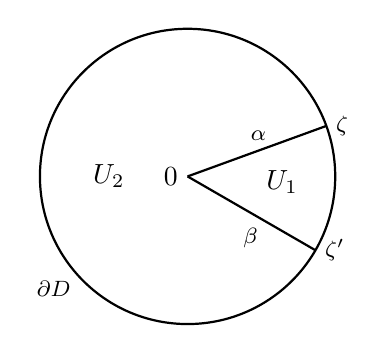
\begin{tikzpicture}
                \draw[thick] (-1.875, 0) arc (180:-180:1.875);
                \draw[thick] ({1.875*cos(20)}, {1.875*sin(20)}) -- (0,0);
                \draw[thick] ({1.875*sqrt(3)/2}, {-1.875/2}) -- (0,0);

                \node[anchor=west] at ({1.875*cos(20)}, {1.875*sin(20)}) {\footnotesize\(\zeta\)};
                \node[anchor=west] at ({1.875*cos(30)}, {1.875*sin(-30)}) {\footnotesize\(\zeta'\)};
                \node[anchor=east] at (0,0) {0};
                \node[anchor=north] at (-1.7, -1.2) {\footnotesize\(\partial\mathbb{D}\)};
                \node[anchor=north] at (0.9, 0.7) {\footnotesize\(\alpha\)};
                \node[anchor=north] at (0.8, -0.53) {\footnotesize\(\beta\)};
                \node[anchor=north] at (1.2, 0.2) {\(U_1\)};
                \node[anchor=center] at (-1, 0) {\(U_2\)};
            \end{tikzpicture}\hfill
            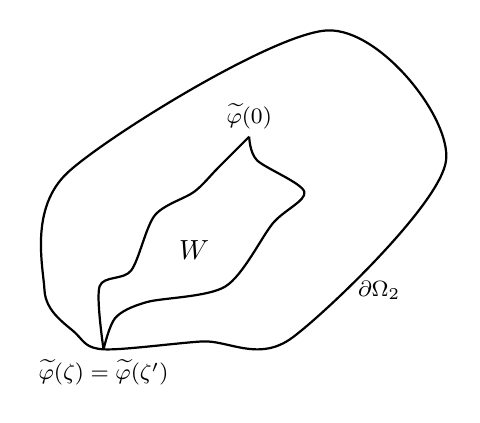
\begin{tikzpicture}
                \draw[thick] plot[smooth cycle] coordinates {
                    (3.6,0.9) (2.1,2.55) (-1.2,0.75) (-1.5,-0.75) (-1.1,-1.3) (-0.75,-1.5) (0.5,-1.4) (1.65,-1.35)
                };
                \draw[thick] plot[smooth] coordinates {
                    (-0.75,-1.5) (-0.8,-0.7)
                    (-0.4,-0.5) (-0.1,0.2) (0.4,0.5)
                    (0.7,0.8) (1.1,1.2)
                };
                \draw[thick] plot[smooth] coordinates {
                    (-0.75,-1.5) (-0.6,-1.1)(-0.2,-0.9)
                    (0.8,-0.7) (1.4,0.1) (1.8,0.5) (1.2,0.9) (1.1,1.2)
                };
                \node[anchor=south] at (1.1,1.17) {\footnotesize\(\widetilde{\varphi}(0)\)};
                \node[anchor=north] at (-0.75,-1.51) {\footnotesize\(\widetilde{\varphi}(\zeta)=\widetilde{\varphi}\qty(\zeta')\)};
                \node[anchor=north] at (0.4,0) {\(W\)};
                \node[anchor=center] at (2.75,-0.75) {\footnotesize\(\partial\Omega_2\)};
            \end{tikzpicture}
            \caption{Two line segments \(\alpha\) and \(\beta\) mapping to a Jordan curve bounding \(W\)}\label{fig:osgoodtaylorcaratheodory_injectivityofextension}
        \end{figure}Notice that \(\widetilde{\varphi}\qty(\mathbb{D})=\Omega_2\), and from the earlier discussion regarding properness, \(\widetilde{\varphi}\qty(S^1)\subseteq\partial\Omega_2\). By the biholomorphy on \(\mathbb{D}\), it thus suffices to show that \(\widetilde{\varphi}{\restriction_{\partial\mathbb{D}}}\) is one-to-one, or that for any two points \(\zeta,\zeta'\in\partial\mathbb{D}\) such that \(\widetilde{\varphi}(\zeta)=\widetilde{\varphi}\qty(\zeta')\), \(\zeta=\zeta'\). Assume, for the sake of contradiction, that \(\zeta\neq\zeta'\). The straight line segment connecting 0 to \(\zeta\) (denoted \(\alpha\)), and the straight line segment joining 0 and \(\zeta'\) (denoted \(\beta\)) then split \(\mathbb{D}\) into two domains \(U_1\) and \(U_2\), and \(\widetilde{\varphi}(\alpha)\cup\widetilde{\varphi}(\beta)\) forms a Jordan curve enclosing some region \(W\). See \cref{fig:osgoodtaylorcaratheodory_injectivityofextension}. By connectivity, either \(U_1\) or \(U_2\) maps to \(W\). Without loss of generality, assume \(\widetilde{\varphi}\qty(U_1)=W\). Then it follows that \[\partial\mathbb{D}\cap\partial U_1\subseteq\partial\Omega_2\cap\partial W=\cbraces{\widetilde{\varphi}(\zeta)}=\cbraces{\widetilde{\varphi}\qty(\zeta')}.\] Then the arc of \(\partial\mathbb{D}\) in \(\partial U_1\) maps to a constant, which by \cref{prop:holomorphicondiskcontinuousonclosureconstantonarcconstancy}, implies that \(\widetilde{\varphi}\) is constant, which is an impossibility. (The same argument is used for \(U_2\))

        Therefore, by the induced contradiction, we must have \(\zeta=\zeta'\), which implies the injectivity of \(\widetilde{\varphi}\).
    \end{proof}
    Thus, the preceding results gives the construction of an injective, continuous extension of \(\varphi\) to \(\overline{\mathbb{D}}\). Moreover, the extension is onto since a continuous function maps compact sets to compact sets.

    Now consider the general case for arbitrary \(\Omega_1\) as in the theorem statement.

    By the preceding results, there exist biholomorphisms \(\varphi_1:\mathbb{D}\to\Omega_1\) and \(\varphi_2:\mathbb{D}\to\Omega_2\), and the Riemann Mapping Theorem (\cref{thm:riemannmapping}) implies the existence of a biholomorphism \(\varphi:\Omega_1\to\Omega_2\). Moreover, \(\varphi_1\) and \(\varphi_2\) extend continuously to \(\widetilde{\varphi}_1\) and \(\widetilde{\varphi}_2\), respectively.

    The restriction \(\widetilde{\varphi}_1{\restriction_{\partial\mathbb{D}}}\) forms a continuous bijection to \(\partial\Omega_1\). We now aim to show that \(\qty(\widetilde{\varphi}_1{\restriction_{\partial\mathbb{D}}})^{-1}\) is continuous. This is in fact a specific case of a famous topological argument that we will avoid. By the final argument of the proof of \cref{cor:osgoodtaylorcaratheodory_continuousextension}, it suffices to show that any sequence \(\cbraces{z_n}_{n\in\mathbb{N}}\subset\partial\Omega_2\) that converges to a point \(z\in\partial\Omega_2\) has a corresponding sequence \(\cbraces{w_n}_{n\in\mathbb{N}}=\cbraces{\qty(\widetilde{\varphi}_1{\restriction_{\partial\mathbb{D}}})^{-1}\qty(z_n)}_{n\in\mathbb{N}}\) in \(\partial\mathbb{D}\) which converges to \(w=\qty(\widetilde{\varphi}_1{\restriction_{\partial\mathbb{D}}})^{-1}(z)\). Assume, for contradiction, that some sequence as labeled above does not converge to \(w\). By the Bolzano--Weierstrass Theorem (\cref{thm:bolzanoweierstrass}), some subsequence of \(\cbraces{w_n}_{n\in\mathbb{N}}\), denoted by \(\cbraces{w_{n_k}}_{k\in\mathbb{N}}\), converges to \(w_\infty\in\partial\mathbb{D}\) (which is not equal to \(w\)). Then \(\widetilde{\varphi}_1\qty(w_{n_k})\to\widetilde{\varphi}_1\qty(w_\infty)\) as \(k\to\infty\) by the continuity of \(\qty(\widetilde{\varphi}_1)\). However, each \(\widetilde{\varphi}_1\qty(w_{n_k})=z_{n_k}\to z=\widetilde{\varphi}_1(w)\). Hence, \(\widetilde{\varphi}_1(w)=\widetilde{\varphi}_1\qty(w_\infty)\) which by injectivity, implies \(w=w_\infty\), which is a contradiction. Thus \(\widetilde{\varphi}_1\) establishes a homeomorphism between \(\overline{\mathbb{D}}\) and \(\overline{\Omega_1}\). A similar deduction gives the same result for \(\widetilde{\varphi}_2\).

    Thus, \(\psi=\varphi_2^{-1}\circ\varphi\circ\varphi_1\in\Aut(\mathbb{D})\), which by \cref{thm:holomorphicautomorphismgrouponunitdisk}, is the composition of a Möbius transformation and a rotation, which extends injectively and continuously to some function \(\widetilde{\psi}\) on \(\overline{\mathbb{D}}\). Thus, we define \(\widetilde{\varphi}=\widetilde{\varphi}_2\circ\widetilde{\psi}\circ\widetilde{\varphi}_1^{-1}\) to be the composition of three continuous functions, defining a continuous extension of \(\varphi\), completing the proof.
\end{proof}
The second case pertaining to \(C^\infty\) boundaries will be proved later. We now entertain the third.
\begin{theorem}\label{thm:osgoodtaylorcaratheodoryrealanalyticboundaries}
    Let \(\Omega_1\) and \(\Omega_2\) be two regions in \(\mathbb{C}\) each bounded by a single real-analytic Jordan curve. Then a biholomorphism \(\varphi:\Omega_1\to\Omega_2\) can be analytically continued to a neighborhood of \(\overline{\Omega_1}\).
\end{theorem}
\begin{proof}
    The Osgood--Taylor--Carathéodory Theorem (\cref{thm:osgoodtaylorcaratheodory}) suffices to extend \(\varphi\) to \(\overline{\Omega_1}\) continuously (continue to denote the extension with \(\varphi\)) such that \(\varphi(\partial\Omega_1)=\partial\Omega_2\).

    Fix \(p\in\partial\Omega_1\) and let \(q=\varphi(p)\in\partial\Omega_2\). Because \(\partial\Omega_1\) is real-analytic, there exists some open interval \(I\) and a real-analytic function \(\eta_1:I\to\partial\Omega_1\) such that \(\eta_1(0)=p\) and \(\eta_1'(t)\neq 0\) for \(t\in I\). By the analytic continuation via power series, \(\eta_1\) can be analytically continued to a region \(N_1\supset I\) on which \(\eta_1'\) does not vanish and \(\eta_1\) is univalent (by \cref{thm:nonvanishingderivativeunivalentonneighborhood}) and conformally maps to a neighborhood \(V_p\ni p\). Then \(\phi=\eta_1^{-1}:V_p\to N_1\) maps \(V_p\cap\partial\Omega_1\) to \(N_1\cap\mathbb{R}\) and \(p\) to 0.

    Similarly, \(V_q\subset\mathbb{C}\) there exists a neighborhood \(V_q\ni q\) and a corresponding complex neighborhood \(N_2\ni 0\) such that \(\eta_2:N_2\to V_q\) is a biholomorphism with \(\eta_2(0)=q\). Define \(\psi=\eta_2^{-1}:V_q\to N_2\) which maps \(V_q\cap\partial\Omega_2\) to \(N_2\cap\mathbb{R}\).

    For \(\psi\circ\varphi\circ\phi^{-1}\) to be defined on some set \(U\), we must have \(\varphi\circ\phi^{-1}(U)\subseteq V_q\), which is satisfied when \(U\subseteq\phi\circ\varphi^{-1}\qty(V_q\cap\overline{\Omega_2})\). The image \(\phi\circ\varphi^{-1}\qty(V_q\cap\partial\Omega_2)\) then is an open interval \(I'\subset\mathbb{R}\) containing 0. Since \(\phi\circ\varphi^{-1}\qty(V_q\cap\Omega_2)\) either lies entirely above (\(\mathbb{H}^+\)) or below (\(\mathbb{H}^-\)) \(\mathbb{R}\), without loss of generality we assume it lies entirely in \(\mathbb{H}^+\). Let \(I''=\qty(N_1\cap\mathbb{R})\cap I'\) and define \(N_1'\subseteq\phi\circ\varphi^{-1}\qty(V_q\cap\Omega_2)\cap N_1\subset\mathbb{H}^+\) to be a new region on which \(\eta_1\) is analytic.

    Then \[\psi\circ\varphi\circ\phi^{-1}\qty(I'')\subseteq\psi\qty(V_q\cap\partial\Omega_2)=N_2\cap\mathbb{R},\] and the composition is of three univalent functions for \(z\in N_1'\) whose ultimate codomain lies either entirely in \(\mathbb{H}^+\) or \(\mathbb{H}^-\) (without loss of generality, we assume \(\mathbb{H}^+\)), and said composition is continuous up to \(I''\).

    By the Schwarz Reflection Principle (\cref{thm:riemannschwarzreflection}), \(\psi\circ\varphi\circ\phi^{-1}\) may be analytically continued from \(N_1'\to\mathbb{H}^+\) to a symmetric domain in \(N_1\), \(U'=N_1\cap\qty(N_1'\cup I''\cup\cbraces{\overline{z}}{z\in N_1'})\to W\subset\mathbb{C}\) biholomorphically (where \(W\) is a neighborhood of 0). Since \(U'\) is a neighborhood of 0, the set defined by \[\psi\circ\varphi\circ\phi^{-1}\qty(U')=W\implies\varphi(V)=\psi^{-1}(W),\] where \(V=\phi^{-1}(U')\) is a neighborhood of \(p\) and \(\psi^{-1}(W)\) is a neighborhood of \(q\). Let \(V'_p\subseteq V\) be an open disk centered at \(p\) and denote the continuation by \(\varphi_p\).

    For every \(z\in\partial\Omega_1\), we may construct a neighborhood \(V'_z\) and a continuation \(\varphi_z\) of \(\varphi\) on \(V'_z\). Now let \(z_1,z_2\in\partial\Omega_1\) be two distinct points such that \(V_{z_1}\cap V_{z_2}\neq\varnothing\). Obviously, \(\varphi_{z_1}\equiv\varphi_{z_2}\) on \(V_{z_1}\cap V_{z_2}\cap\overline{\Omega_1}\neq\varnothing\). Hence the Identity Theorem (\cref{thm:identity}) implies that \(\varphi_{z_1}\equiv\varphi_{z_2}\) on all of \(V_{z_1}\cap V_{z_2}\).

    Therefore, the local continuations \(\cbraces{\varphi_z}_{z\in\partial\Omega_1}\) agree on overlaps and concatenate together to define a single-valued holomorphic extension of \(\varphi\) to a neighborhood of \(\overline{\Omega_1}\).
\end{proof}
